\documentclass{article}

\usepackage{amsmath}
\usepackage{nicefrac}
\usepackage{diffcoeff}
\usepackage{amsmath}
\usepackage{tikz}
\usepackage{subcaption}
\usepackage{graphicx}
\usepackage{float}
\usepackage{hyperref}

\tikzstyle{box}=[draw, fill=red!20, minimum size=2em]

\title{A Dynamical Model of Social Movements on Social Media}
\author{
    Alyssa Baksh, 
    Ciaran Neely,
    Gianna Biino,
    Zaheer Mohideen
}

\begin{document}

    \maketitle

    \section{Abstract}
    This paper explores a model of how social movements progress on social media. Social movements influence our everyday lives and can explain many sociological phenomena \cite{diani_networks_2013}. With the rise of social media, human interactions have evolved and can to be analyzed in new ways \cite{kidd_social_2016}. Using a mathematical SEIR model the number of people actively participating, being aware of the movement and not knowing about it are calculated over a time span of several weeks. With a few assumptions it is possible to analyze the parameters important to the spread of social movements on social media. Looking at specific cases while keeping the rest of the parameters constant we could see how they influence the death or continuation of social movements. 
    
    \section{Introduction}
    Social networks and movements have been a crucial part of society and open a window to explaining many phenomena such as herd mentality and what causes individuals to participate in social movements \cite{diani_networks_2013}. Opinions, values, and grievances are often not enough to induce actions. Connections to people participating in a social movement are generally needed to make people act \cite{small_movements_2021}. Hence it is reasonable to assume that affiliation with a social movement will spread through the population similarly to how a virus might.
    
    Social movements are a sociological analytical concept defined as networks of interactions between different individuals, groups and organizations, who are engaged in political or cultural conflicts, on the basis of a shared collective identity. The important aspects that need to be considered when defining the dynamics of a social movement are: 
    \begin{itemize}
    \item It needs to be a network based on informal interactions between groups and/or organisations and individuals.
    \item It needs to contain a collective solidarity and shared beliefs.
    \item It needs to engage in conflicts, cultural or political, and promote or dispute social change.
    \item  For the majority of it, the action needs to be outside of routine and institutional procedures of social life.
    \end{itemize}
    Thanks to the broad definition of these aspects, the concept can be adapted to specific examples. If, for example, one study focuses on a global anti-systemic social movement another will focus on a social movement supporting a local system and opposing changes to it. \cite{diani_concept_1992}
    
    With the recent emergence of social media networks, the studies of social movements have evolved again, prompting further inquiries on the topic\cite{kumar_structure_2006}.
    
    Many studies have started to compare how movements founded upon social media compare to those in the past that weren't\cite{kidd_social_2016}. For example, the transnational movement in Italy was analyzed to see how digital media like Facebook was used by activists to spread their message, considering the number of posts, likes and comments over the  years \cite{pavan_digital_2019}. 
    
    Other studies looked at international movements. For example, one on the \textit{Black Lives Matter} movement, considering multiple social media platforms and the level of engagement of accounts. This study also discussed the limitations of social media. On one hand, traditional forms of organization still play an important role to sustain and build a movement. On the other hand, through the accessibility of social media, it is hard to maintain the actual goal and values of a movement, since many people can participate who might have different goals in mind. It is also easier for individuals to contradict the movement online by spreading opposing messages. The benefits of social media however, outweigh the costs, as it allows for a bigger scaling of social movements and a broader audience can be reached. \cite{mundt_scaling_2018}

    Using mathematical models, we aim to gain a deeper understanding how social movements progress with time over social media and if we can find a pattern between social movements and various parameters Specifically, we hope to find which parameters and what values are necessary for a social movement to spread and how can they be used as tools in order to spread a message.

    \section{Methods}
   
    %Let $I(t)$ be the number of people engaged in the social movement at time t, and let $E(t)$ be the number of social media users who are aware of the movement at time t. Let $S(t)$ be the number of active social media users at time t who are not aware of the movement at all, and let $P(t)$ be the population of the community where the social movement is taking place. 

    \begin{figure}
        \centering
        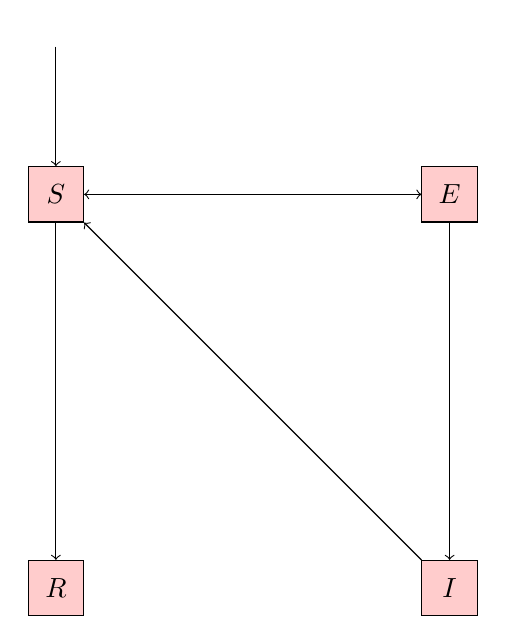
\begin{tikzpicture}
            \node [box] (S) {$S$};
            \node [box, right of=S, node distance=5cm] (E) {$E$};
            \node [box, below of=E, node distance=5cm] (I) {$I$};
            \node [box, below of=S, node distance=5cm] (R) {$R$};
            \node [above of=S, node distance=2cm] (out) {$ $};
            \path[<->] (S) edge (E);
            \path[->] (E) edge (I);
            \path[->] (I) edge (S);
            \path[->] (S) edge (R);
            \path[->] (out) edge (S);
        \end{tikzpicture}
        
        \caption{A diagram of the model}
        \label{fig:model_diagram}
    \end{figure}
    
    We relate our model (Figure \ref{fig:model_diagram}, Equation \ref{meq_main}) to a type of SEIR disease model where $I(t)$ is the number of infected individuals, who are able to spread the disease to $S(t)$ who are the number of susceptible people. In our case, this would mean people actively engaged in the movement would be exposing social media users through posts. $E(t)$ acts as the exposed population, those who have come in contact with the disease, or in our case, those who have in come contact with the social movement by seeing social media posts about it, but who are not yet actively involved. Similarly to how exposed individuals have a chance of becoming infected or going back to being susceptible, in our model, those who are exposed to the movement can decide if they wish to actively engage in it or go back to being a part of the susceptible, $S(t)$.

    While no particular study relates the SEIR model to social movements and in particular social media, there are a few studies which involve analysing the use of social media alongside controlling the spread of diseases. Our model uses a similar analysis and techniques as some of these articles \cite{du_how_2021}\cite{choi_effects_2017}.
    
    In our model we do not have an $R(t)$, recovered members, because we want to focus on how efficiently people are joining the movement when exposed to social media, rather than focusing on those who are ``recovering" from it. Moreover, our model also includes density dependence for Equation \ref{eq:main_i}, as $I(t)$ increases, that means there are more infected individuals, and thus there are fewer susceptible people to expose/infect, and thus $I'(t)$ would decrease depending on the population.
    
    Before we start stating our equations, we need to clarify some assumptions that our model makes when taking the population and behavior of people into consideration.

    \subsection{Assumptions}
    
    Some of the assumptions we will make are listed here:
    \begin{enumerate}
    \item  Everyone has equal access to social media, and our $S(t)$ only focuses on active social media users.
    
    \item We won't consider a particular social media platform or consider different platforms as a parameter, but rather social media in general. 
    
    \item We divide the population into two parts, labelling those who use social media as $S(t)$ and those won't don't as $P(t)$. 
    
    \item We consider a closed population which means people who are not concerned about movement, will not share posts on social media. 
    
    \item The movement does not experience significant external interventions or disruptions. For example, there is not an opposing movement that is causing members to leave the other. 
    
    \item The movement does not have significant internal divisions or conflicts that affect its growth and spread.
    
    \item The platform used for the movement has a stable user base and does not experience significant changes in its user base or functionality.

    \item The population of the community where the movement is taking place is relatively stable and does not experience significant demographic changes.

    \item Social media overload can cause people to disengage from the movement and the platform.
    
    \item  The only way people can engage or become aware of the movement is through social media, particularly through posts that are being sent only by people already actively engaging in the movement, called infleuncers. 
    
    \item  After some time posts tend to lost traction and no longer become trending. Thus, there can only exist a certain number of trending posts at any given period of time $t$. That is, $F(t)$ is a bounded function with maximum equal to $k_8$. 

    \item Influencers are all equally influential online.

    \item People are equally likely to see trending posts. Once they do, they immediately become ``exposed" and then decide if they would like to join the movement or not. 
    
    \item People who leave the movement or decide not to join the movement after becoming exposed still use social media, so are then part of $S(t)$. We assume they just forget their recent exposure/involvement with the movement and are completely unaware of it until they are exposed another time. 
    
    \end{enumerate}
    \subsection{Model Equations}
     Let $N$ be the total population of the community where the social movement is taking place.
     Let $I(t)$ be the number of people engaged in the social movement at time $t$, let $E(t)$ be the number of social media users who are aware of the movement at time $t$, let $R(t)$ be the number of people recovering from using social media, meaning they stop using it completely, thus it's a particular subset of $P(t)$. Let $S(t)$ be the number of active social media users at time $t$, let $P(t)$ be the population of the community that does not use social media and let $F(t)$ is the number of trending posts related to the movement at time $t$.
    
    \begin{subequations}
    \begin{align}            
        \diff St &= k_6 P(t) + k_2I(t) + k_5E(t) - k_3 {S(t)I(t)}- k_7S(t)-k_4 F(t)S(t)\label{eq:main_s}
        \\[10pt]
        \diff Et &= k_3 I(t)S(t) + k_4 F(t) S(t) - k_5E(t) - k_1E(t)\left[1 - \frac{I(t)}{S(t)}\right] \label{eq:main_e}
        \\[10pt]
        \diff It &= k_1 E(t) \left[1 - \frac{I(t)}{S(t)}\right] - k_2I(t)\label{eq:main_i}
        \\[10pt]
        \diff Rt &= k_7S(t) \label{eq:main_r}
    \end{align}
    \label{meq_main}
    \end{subequations}
    
    where
    \begin{subequations}
    \begin{align}
        P(t) &= N - S(t) - E(t) - I(t)
        \\[10pt]
        F(t) &= k_8\sqrt{\frac{I(t)} N}
    \end{align}
    \end{subequations}

    and where
    \begin{itemize}
        \item $k_1$ is the inverse of the minimum expected number of weeks it takes for a person to go from $E$ to $I$. In other words the time it takes for an exposed individual to become actively involved;
        \item $k_2$ is the inverse of the expected number of weeks for an active member to lose interest and leave the movement;
        \item $k_3$ is the rate at which social media users become exposed and are aware of the movement (measured in $[1/{(people\times weeks)}]$);
        \item $k_4$ is the rate at which influencers promote the movement and thus make more people aware of the movement; 
        \item $k_5$ is the inverse of the expected number of weeks an exposed person loses interest and disengages from the movement;
        \item $k_6$ is the rate at which the non-social media using population joins social media (measured in $[1/{weeks}]$);
        \item $k_7$ is the expected number of weeks for a person to leave the platform due to social media overload or other factors; and
        \item $k_8$ is the maximum number of trending posts that can be absorbed by a single person (measured in $[posts]$) (a phenomenon called the law of diminishing returns \cite{dhaoui_brand_2021}).
    \end{itemize}

    Equation \ref{eq:main_s} describes most generally how the number of active social media users (excluding those in $E$ and $I$) changes over time. The number of users is increasing due to social media adoption, but it is also subject to a rate of decline due to social media overload or other factors. We model this as proportional to the product of the number of social media users and the number of people engaged in the movement relative to the population size. 

    Equation \ref{eq:main_e} describes how the awareness of the movement changes over time, with the number of social media users becoming aware of it proportional to the number of users who are already aware of it, as well as the rate at which influencers promote it. The rate of awareness is also subject to a rate of disengagement due to social media overload, which is proportional to the product of the number of social media users and the number of people engaged in the movement. 
    
    Equation \ref{eq:main_i} describes how the size of the movement changes over time, with the number of people becoming engaged in the movement being proportional to the number of social media users who are aware of it and the available population who may join the movement, but also subject to a rate of disengagement. 
    

    Finally, Equation \ref{eq:main_r} describes how social media users the platform, with the rate simply being proportional to those not actively involved in a movement that would keep them invested.
 

    \section{Results}
    
    There are certain cases we can take into consideration and analyze depending on the parameters $k_1$ through $k_8$. In order to simplify the analysis the parameters not relevant to the specific case are set to a default value which is equal to $0.5$. If the default value is changed, the pattern of the graph is scaled inversely to the change of the $k$-value.
    The time length considered in each case varies in the number of months, such that the graphs can be easily interpreted. The initial distribution of the number of people to each category is the following: $E$ starts at $0$, $S$ starts with 5 numbers equally spaced out in between $0.1$ and $0.9$ and I starts with 5 numbers equally spaced out in between $0.005$ and $0.1$.


    \subsubsection*{Case 1: Rapid growth followed by quick decline, $k_1 \gg k_5$} \normalfont
    Assuming that $k_1$  is much greater than $k_5$, the social movement is likely to experience rapid growth as more and more social media users become engaged and stay involved. However, if $k_2$ (rate of actively engaged people leaving the movement) is also high, the movement could fizzle out quickly as actively engaged individuals leave. If it was low, the movement could continue to grow and attract even more engaged individuals.

    Simulating this with a low $k_2$-value (Figure \ref{fig:case1_lowk2}) we see an increasing number of people aware and actively involved in the movement stabilizing at around $0.2$, with the actively involved people stabilizing at a slightly higher frequency. The number of people who are unaware of the stabilises at a frequency of around $30\%$ of the population.
    
    Using a high $k_2$-value on the other hand (Figure \ref{fig:case1_highk2}), the movement dies down after only a few weeks, so the number of people who know about it goes to zero. The number of people who are on social media but are unfamiliar with the movement stabilizes at around $0.5$, because there will always be a certain amount of people who will not be on social media and the rate of people leaving and joining social media have the same values. The stabilization also occurs much quicker than in Figure \ref{fig:case1_lowk2}. 
    
    \subsubsection*{Interpretation}  While the movement experiences rapid growth in its initial stages, the frequencies stabilize after a few weeks. The limit depends on $k_2$. If $k_2$ is low all three categories stabilize at a limit bigger than zero. However, if $k_2$ is high the movement dies out after only a few weeks. Therefore, it is important to strike a balance between retaining engaged individuals and allowing individuals who no longer align with the movement's goals to leave, in order to ensure the long-term success and impact of the movement.
    
    \begin{figure}[H]

        \centering
        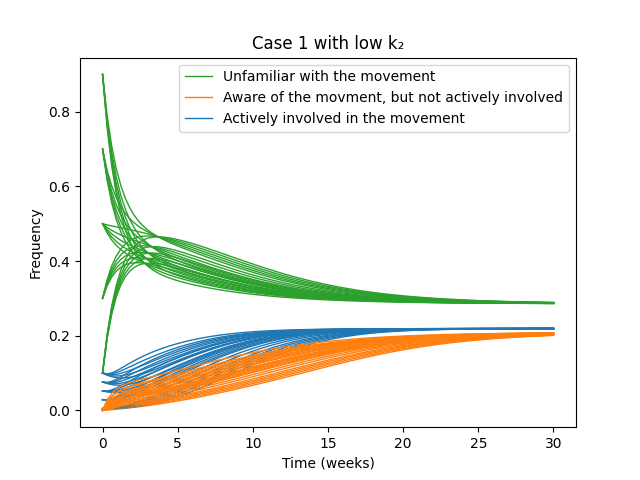
\includegraphics[width=\textwidth]{simulation/plots/case1-lowk2.png}   
        \caption{Many overlaid time series of the model involving \mbox{$k_1=.9$} , \mbox{$k_2=.2$}, \mbox{$k_5=.1$}}
        \label{fig:case1_lowk2}
    \end{figure}

    \begin{figure}[H]

        \centering
        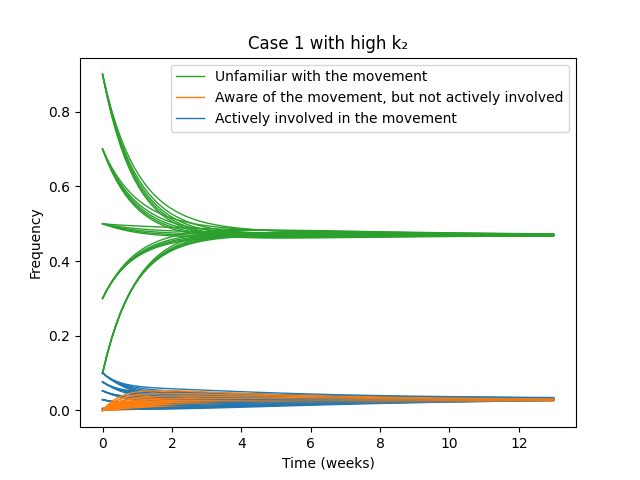
\includegraphics[width=\textwidth]{simulation/plots/case1-highk2.png}   
        \caption{Many overlaid time series of the model involving \mbox{$k_1=.9$}, \mbox{$k_2=.8$}, \mbox{$k_5=.1$}}
        \label{fig:case1_highk2}
    \end{figure}


    \subsubsection*{Case 2: Struggling to gain traction, $k_3 < k_1$ and $k_3 < k_5$}
    Assuming that $k_3$ is much smaller than $k_1$ and $k_5$, the social movement may struggle to gain traction as social media users are not becoming aware of the movement at a fast enough rate, and exposed individuals are disengaging quickly. 

    In Figure \ref{fig:case2_lowk4} similar to Case 1 with a high $k_2$ the movement dies down and the frequency of people on social media who are unfamiliar with the movement stabilizes again at around $0.5$.
    
    \subsubsection*{Interpretation} The movement  struggles to gain momentum and grow and eventually it dies out. However, if the rate at which influencers promote the movement ($k_4$) is high, then the movement could still gain traction and attract more engaged individuals, despite a slow initial growth. After trying, we have concluded, that the $k_4$ value alone is not sufficient to save the moment, the values of other parameters need to be adjusted as well. Therefore, it is important to consider both the rate of exposure to the movement and the influence of key individuals in promoting and sustaining momentum for the movement.
    
    \begin{figure}[H]

        \centering
        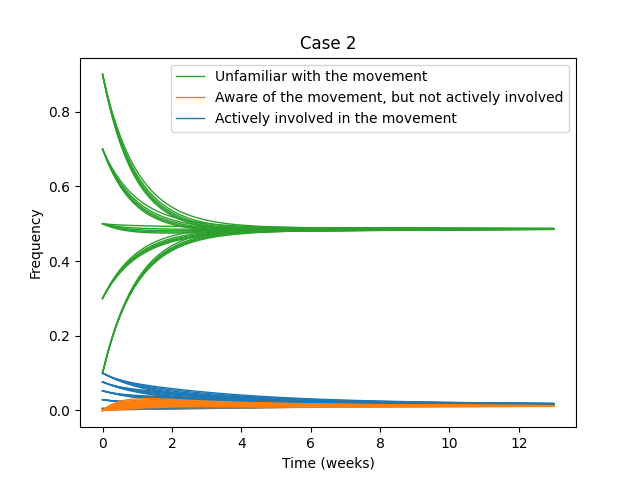
\includegraphics[width=\textwidth]{simulation/plots/case2-lowk4.png}   
        \caption{Many overlaid time series of the model involving \mbox{$k_1=.7$}, \mbox{$k_3=.1$}, \mbox{$k_5=.7$}}
        \label{fig:case2_lowk4}
    \end{figure}
    
    \subsubsection*{Case 3: Influencers driving movement forward, $k_4 > k_5$} \normalfont
 
     In this case, influencers could play a key role in driving the movement forward by promoting it frequently. The movement is more likely to gain momentum and have a lasting impact. This is because influencers can help sustain engagement and encourage continued participation even as individuals may be exposed to negative or disengaging factors. By promoting the movement and highlighting its benefits and impact, influencers can motivate individuals to become engaged and invested in the movement. This can help sustain participation over time and mitigate the potential negative effects of disengagement on exposed individuals.

    In Figure \ref{fig:case3} the frequency of people unfamiliar with the movement stabilize at around $0.4$, whereas the frequencies of the other two groups stabilize at around $0.1$. Compared to Figure \ref{fig:case1_lowk2} this time the limit of the frequency of people who are actively involved in the movement is a bit below the limit for those who are aware but not actively involved.
     
    \subsubsection*{Interpretation} The movement continues to thrive, even if some exposed individuals disengage. This case underscores the importance of the role of influencers in promoting a social movement and sustaining engagement over time. 

    \begin{figure}[H]

        \centering
        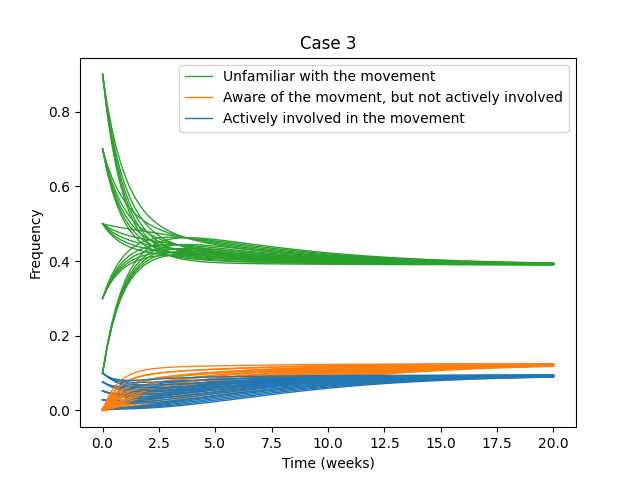
\includegraphics[width=\textwidth]{simulation/plots/case3.png}   
        \caption{Many overlaid time series of the model involving \mbox{$k_4=.9$}, \mbox{$k_5=.2$}}
        \label{fig:case3}
    \end{figure}


    \subsubsection*{Case 4: Sudden spike in engagement but high risk of burnout, $k_6 > k_3$ \normalfont{and} $k_6 > k_5$}
   In this case, the movement has the potential to rapidly gain momentum and reach a wide audience. As more individuals in the community join social media, they become exposed to the movement and may become engaged and invested in its goals and objectives. This can help sustain momentum and encourage continued participation, particularly if efforts are made to retain engaged individuals and address negative factors contributing to disengagement. 
   
   However, it is also important to consider the potential challenges associated with rapid growth and expansion. As the movement gains momentum and reaches a wider audience, it may become more difficult to maintain cohesion and direction, particularly if there are diverse opinions and perspectives  participants.
   
    \subsubsection*{Interpretation} In summary,  this case highlights the potential benefits and challenges associated with rapid growth and expansion in a social movement. By complementing efforts to increase visibility and engagement with broader strategies to manage growth and maintain cohesion, social movements can maximize their impact and reach a wider audience.
    This case only concerns itself conceptually with the number of people. Therefore there is no graph to represent it as it will stabilize itself at similar ratios as the other graphs.

    \subsubsection*{Case 5: $k_3 > k_6$}
    In this case, the movement may struggle to gain traction and expand its reach beyond initial participants.
    
    While efforts to raise awareness of the movement  existing social media users may help to generate initial interest and support, the movement may struggle to expand its reach beyond this initial group without effective strategies for engaging individuals who are not already using social media.
    
    In such a scenario, it may be useful to consider strategies for increasing social media adoption  non-users, such as targeted advertising or outreach efforts. Additionally, efforts to establish partnerships with organizations and groups outside of social media can help to generate broader support and reach individuals who may not be engaged through social media alone.

    As can be seen in Figure \ref{fig:case5} the awareness of the movement increases initially but slowly dies down, as predicted. What is interesting in this case, is that even though $k_3$ is much higher than $k_6$ not all of the social media users will be familiar with the movement. This might be due to the parameters $k_2$ and $k_5$ of people leaving the movement, whether they were active or not. Since both of these parameters are relatively high (default value of $0.5$) they have a large influence on the group sizes. 
    
    \subsubsection*{Interpretation}
    Depending on multiple parameters, the movement is likely to plateau and fails to reach new individuals. Since our model allows for people to loose and regain interest in the movement it will stabilize after a some weeks. This case highlights the potential challenges associated with relying solely on social media to promote and sustain a social movement. By complementing efforts to increase awareness and engagement on social media with strategies for engaging non-users and establishing partnerships with organizations outside of social media, social movements can maximize their impact and expand their reach beyond initial participants.

    \begin{figure}[H]

        \centering
        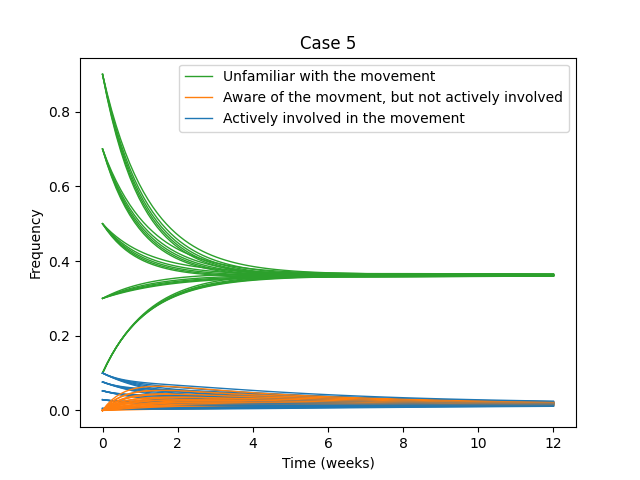
\includegraphics[width=\textwidth]{simulation/plots/case5.png}   
        \caption{Many overlaid time series of the model involving \mbox{$k_3=.8$}, \mbox{$k_6=.3$}}
        \label{fig:case5}
    \end{figure}


    \subsubsection*{Case 6: $k_4 > k_5$ \normalfont{and} $k_8 > k_7$}
    In this case, influencers are effectively promoting the movement ($k_4 > k_5$) and social media users are leaving the platform at a slower rate than they are joining it ($k_8 > k_7$). This means that while social media may be overwhelming some users, it's still an effective tool for spreading awareness and engaging new supporters.

    As can be seen in Figure \ref{fig:case6} the three groups stabilize after a few weeks at non-zero values. This shows that the social movement will be continued on at that level for some time until one of the parameters changes.
    \subsubsection*{Interpretation}
    The movement is likely to continue growing in popularity, but social media may need to find ways to reduce user overload and keep existing users engaged. In real life, the parameters are probably going to change after some time, which means that the system will never stabilize.

    \begin{figure}[H]

        \centering
        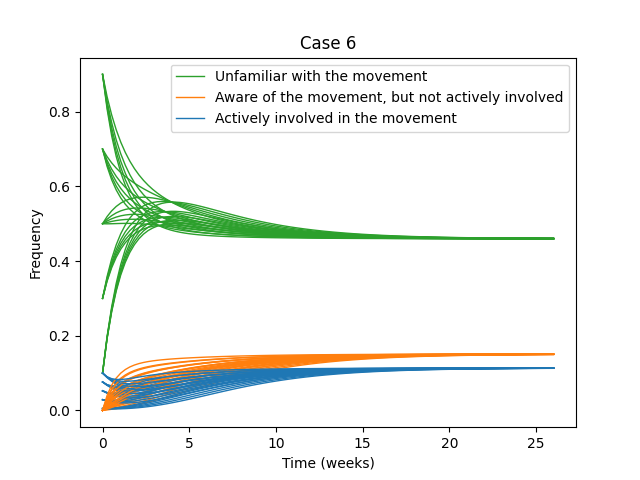
\includegraphics[width=\textwidth]{simulation/plots/case6.png}   
        \caption{Many overlaid time series of the model involving \mbox{$k_4=.7$}, \mbox{$k_5=.3$}, \mbox{$k_7=.3$}, \mbox{$k_8=.7$}}
        \label{fig:case6}
    \end{figure}

    \section{Discussion}
    

    Social movements are much more dynamic than shown in our model. They can grow or die down within hours to years, depending on how the circumstances change, how the movement and its goals is interacted with as a society and not only on social media \cite{hiller_reconceptualization_1975}. Our model simplifies this complex movement and puts it into a world without any exterior influences that could change the parameters. This means, that the most ``realistic" part of the time series might only be the first week or so since the real world never gives a specific movement enough time to stabilize itself.
    
    After working with and interpreting a few cases for our model, we observe that our functions all seem to stabilize, but just with varying speeds and limits. This is to be expected as our main goal was to analyze how quickly social movements grow with varying social media exposure, influencing power, and active social media use rather than working with stability cases like what we've seen in our lectures. 
    
    From the case analysis graphs, we can see that social media does in fact play a role in boosting the growth of social movements, but only when accompanied by other factors. For instance, if we have a large number of influencers/infected individuals but their rate of infecting is very low for various reasons such as bad quality posts or not reaching the proper demographic, then their efforts won't be as effective. Thus, if politicians or those in a social movement decide to use their resources on social media, they have to ensure that it's effective and properly correlates to the demographics that they're trying to persuade. 

    We conclude that $k_4$ does play a significant noticeable role in promoting/inhibiting movement growth. This makes sense in a social setting as having a high rate of influencers being able to promote the movement directly affects the rate at which users join the movement. $k_2$ also seemed to affect the limit at which our graphs stabilised like with case 1 which again correlates 

    A few ways to increase the accuracy of our results would be varying the constant parameters $k_1$ to $k_8$ in each of the cases. For accuracy purposes, we should conduct all the cases with varying case parameters as well, for instance, having $k_1=k_5 = 0.99$ and $k_3 = 0.01$ in case 2, etc. However, after analyzing these different cases, there didn't seem to be any significant differences from what we already found. Another suggestion would be to conduct the study with a base value of $0.2$ or $0.7$ instead of just $0.5$. This would help us analyze how fast social movements grow and stabilize with varying exposure to social media. A more accurate model would be to add another variable or change the parameters to variables, as it would be easier to model the changes within the movement and the world that surrounds it.

    \newpage
    \bibliographystyle{plain}
    \bibliography{references}
    \section{Appendix}
    Source code for this document and all its figures is available at \url{https://github.com/cicilapetitesorciere/Social-Movements-Report}
\end{document}